\documentclass{acm_proc_article-sp}
\bibliographystyle{unsrt}

\begin{document}

\title{Cellular Automata for Molecular Life Games}
\numberofauthors{1}
\author{
% 1st. author
%\alignauthor
%Alan S. Wang\\
%       \affaddr{Department of Bioengineering}\\
%       \affaddr{University of California}\\
%       \affaddr{California, Berkeley}\\
% 2nd. author
\alignauthor
Ian Holmes\\
       \affaddr{Department of Bioengineering}\\
       \affaddr{University of California}\\
       \affaddr{California, Berkeley}\\
       \email{ihh@berkeley.edu}
}
\date{30 November, 2013}

\maketitle
\begin{abstract}
An experimental turn-based multiplayer game framework for mobile devices is described.
Using cellular automata, the framework implements models
of condensed-matter physics, mathematical biology,
and the computational study of artificial life.
\end{abstract}

% A category with the (minimum) three required fields
%\category{H.4}{Information Systems Applications}{Miscellaneous}
%A category including the fourth, optional field follows...
%\category{D.2.8}{Software Engineering}{Metrics}[complexity measures, performance measures]


\section{Introduction}

Cellular automata ({\em CA}) are a versatile platform for a wide
range of models from physics, biology and chemistry\cite{Schiff2007}.
They are also widely employed in the study of artificial computational life ({\em A-Life}).
CAs have supported diverse A-Life designs,
whether inspired by electronic circuits\cite{VonNeumannBook,Wireworld},
cells, insects, or other macro-biological systems\cite{ConwaysLife,Langton1986},
or kinematic systems\cite{Stevens2011}.

Another type of A-Life involves code that is placed under direct pressure to evolve.
The ancestor of all these is the competitive programming game CoreWar
\cite{CoreWarGuidelines84,BarkleyWaitSchmidtCoreWar2004}.
Successors Tierra\cite{Tierra} and Avida\cite{Avida} more directly investigate the
behavior of genetic algorithms.

With the goal of investigating systems such as this and developing associated game mechanics,
the PixelZoo game engine has been designed to support
a persistent, multiplayer, computationally-dense world using CA.
This paper reviews the design and progress of PixelZoo,
including implementation of several biophysically-inspired models
simulating polymer and RNA folding kinetics.

CAs have been used as game devices before,
as in Sim City, %\cite{SimCity},
Dwarf Fortress, %\cite{DwarfFortress},
and Minecraft. %\cite{Minecraft}.
They have also been used in software toys and art such as
PowderToy %\cite{PowderToy}
and CAPOW. %\cite{RuckerCAPOW}.
There are many freely available engines to simulate various kinds of CA, such as Golly. %\cite{Golly}.
In relation to such prior efforts, PixelZoo
(i) is more focused on molecular biophysics and evolution,
(ii) is intended to be a game rather than a simulator.

\subsection{Molecular Evolution Models}

One of the best-studied models of the origin of life is the ``RNA World'' hypothesis,
which posits that RNA molecules were the first self-replicating entities\cite{Woese1967}.
The chemistry of RNA naturally favors self-replication under favorable conditions,
such as spatial concentration of the necessary ingredients.
Early life has been conjectured to involve concentration of RNA precursors within {\em micelles}:
essentially, spontaneously-forming bubbles of amphiphilic (detergent) molecules.

Testing hypotheses about the distant past is difficult, but synthetic life experiments
have lent plausibility to the RNA World\cite{PaulJoyce2002}.
RNA has been discussed in the context of A-Life models\cite{journals/alife/Schuster94}.
Biophysicists have devoted considerable attention to CA-like lattice models of RNA folding
\cite{LeoniVanderzande2003,JostEveraers2010,ZaraPretti2007,GillespieMayneJiang2009},
following earlier studies of protein folding on the lattice \cite{Dill1985,PandeRokhsar1999}.

\section{Simulation}

The PixelZoo board is
an $S \times S \times D$ slab of the cubic lattice,
requiring $16S^2 D$ bytes on a 64-bit architecture (128 bits/cell),
plus any Scheme programs that are attached.
Gameplay is generally restricted to a thin 2D slab ($D \leq 2$).

In a diffusion-based simulation, speed is paramount.
The PixelZoo language exposes a fast low-level state machine for majority usage during play,
generalizing the concept of the CA state lookup table to allow partial matching
and rewriting of bitfields in the local lattice neighborhood (but not much else).
There is also a high-level functional language (Scheme) available both for generation of low-level instructions,
and for occasional in-game scripting usage.

\subsection{Low-Level Virtual State Machine}

The low-level state machine supports two alternatives for periodic updates:
synchronous (fixed time interval between calls)
and asynchronous (exponentially-distributed time between calls, scaled by particle's update rate).
The random number generator is a Mersenne twister, and supports replay.

Cells can address their local neighborhood.
There are 64 bits of state per cell,
plus a pointer to opaque storage that can only be accessed via the higher-level scripting language.

The 64 bits of state are divided into bitfields.
16 bits are given over to a type field, determining how the cell will be updated.
The remaining 48 bits are used as dynamic storage; the division into bitfields depends on the type,
with some universal restrictions (e.g. bitfields cannot straddle a 32-bit boundary).

The 16-bit type field selects the global program to update the cell and its neighborhood,
and specifies the naming and sizing scheme for dynamic bitfields.

The virtual machine resembles an ultra-minimal subset of a typical CISC register-machine architecture.
The instruction set is low-level, recognizably close to ARM\cite{seal00} and not too far from CoreWar's RedCode\cite{CoreWarGuidelines84}.
The instructions can be quickly interpreted from or implemented in C, and will be optimized reasonably well by C compilers.
Such details of the implementation are left opaque by design.
Code written for the low-level state machine cannot reflect on or modify its own global program.
\begin{center}
\fbox{ \parbox{.9\columnwidth}{
{\bf INSTRUCTION SET.}
The following minimalistic operations were designed with the goal of fast simulation of particles and polymers.
Excluding random numbers and Scheme,
the core instructions are readily compiled to C
({\tt switch}, {\tt if}, {\tt goto}, integer math)
or directly to a RISC instruction set like ARM\cite{seal00} ({\tt LDR}, {\tt STR}, {\tt ADD}, {\tt CMP}, {\tt B}).
\\
{\tt Load-Add-Store}: loads value from source bitfield, adds operand, and stores result in destination bitfield: can optionally move or destroy the opaque S-expression storage.
\\
{\tt Load-Compare-Branch}: reads value from bitfield, compares to operand, branches conditionally.
\\
{\tt Load-Switch}: analogous to C's {\tt switch}: reads bitfield, then dispatches control based on bitfield value.
\\
{\tt Load-Register}: places a numeric constant into a register. Used in combination with indirect addressing modes of other
instructions.
\\
{\tt Branch-Goto}: branches to labeled routine.
\\
{\tt Branch-Random}: branches conditional on random bit.
\\
{\tt Branch-Neighbor}: yields to neighbor cell's program.
\\
{\tt Call-Script}: yields to arbitrary Scheme function.
} }
\end{center}
It bears re-emphasis that the prime design criterion of this instruction set is to {\em limit} the expressive power of programs
to something comparable to state lookup tables.
Control flow is monotonic: there is no stack, and no gosub or return keywords.
Branches always go forward, so loops are explicitly prohibited.
Any program is a Directed Acyclic Graph (DAG) of finite determinable length.
It is thus easy for a server to analyze player-designed programs and maintain strong performance guarantees.
There is enough flexibility for players to implement novel material properties in the CA,
as well as more sophisticated computational behaviors (e.g. Turing machines, Langton ants, Wireworld-type circuits).

\subsubsection{Addressing Modes}

The machine supports several addressing modes for memory locations and operands.
{\em Immediate operands} allows specification of constants within the code,
while {\em register operands} allows these constants to be loaded into registers first (enabling some code re-use).

Memory addressing is local to the neighborhood cell.
{\em Direct addressing} requires bitfield addresses and relative cell co-ordinates to be hardwired into the code,
while in {\em indirect addressing} these are specified by register values at run time.

In principle, indirect or register addressing are not necessary to implement polymers:
we can explicitly enumerate all cases via immediate and direct addressing.
In practice, it's useful to allow some indirect/register addressing,
to reduce program sizes via re-use of subroutine-like code.

\subsubsection{Assembly Language}

The virtual machine may be programmed directly in XML, but this XML is more usually generated using
a Scheme-based assembly language.

The assembler has a built-in library for programming CAs on the square lattice:
replicating patterns over Moore or von Neumann neighborhoods,
implementing reaction-diffusion models, implementing turtle-type agents, and so on.

Selected functions from this library are exposed to the player,
to facilitate game design (e.g. diffusions, turtles) and reduce program sizes.

\subsection{Higher-Level Functions}

As well as being used at assembly time to specify macros,
Scheme functions can be invoked dynamically by {\tt Call-Script}
for higher-level supervisory functions of an occasional nature,
such as path-finding or goal-directed planning.
These features are restricted to game designers.

An optional S-expression can be associated with any cell for dynamic storage associated with the agent scripts.
This storage is opaque to the state machine: there is one instruction ({\tt Load-Add-Store}) that, when rewriting the type field of a cell, is allowed to relocate or destroy the S-expression associated with it.
Other than this, the low-level machine may not copy, create, read or modify cell S-expressions.
In contrast, the Scheme supervisor has access to the state machine environment, board API, and multiplayer client API.

The polymers, RNA molecules, and other models described here
 (Sections~\ref{sec:PolymerStateMachines} through~\ref{sec:AgentStateMachines})
 do not require Scheme scripting, only Scheme assembly language generation (which is a one-time cost).

\subsection{Polymer State Machines}
\label{sec:PolymerStateMachines}

The fundamental biological molecules (DNA, RNA and proteins) are all polymers.
In 2D, closed-loop polymers can also represent thermodynamically fluctuating enclosures like micelles.

Drawing on the stochastic physics of polymers \cite{DoiEdwards1988}
and their simulation on lattices \cite{PhysRevLett.64.1915,journals/pc/OstrovskyCSB01},
PixelZoo uses a bidirectionally-linked list model.
The possible configurations of a cell, its neighbors, and adjacent empty spaces must
be explicitly enumerated, as shown in Figure~\ref{fig:polymer}.

\begin{figure}
\fbox{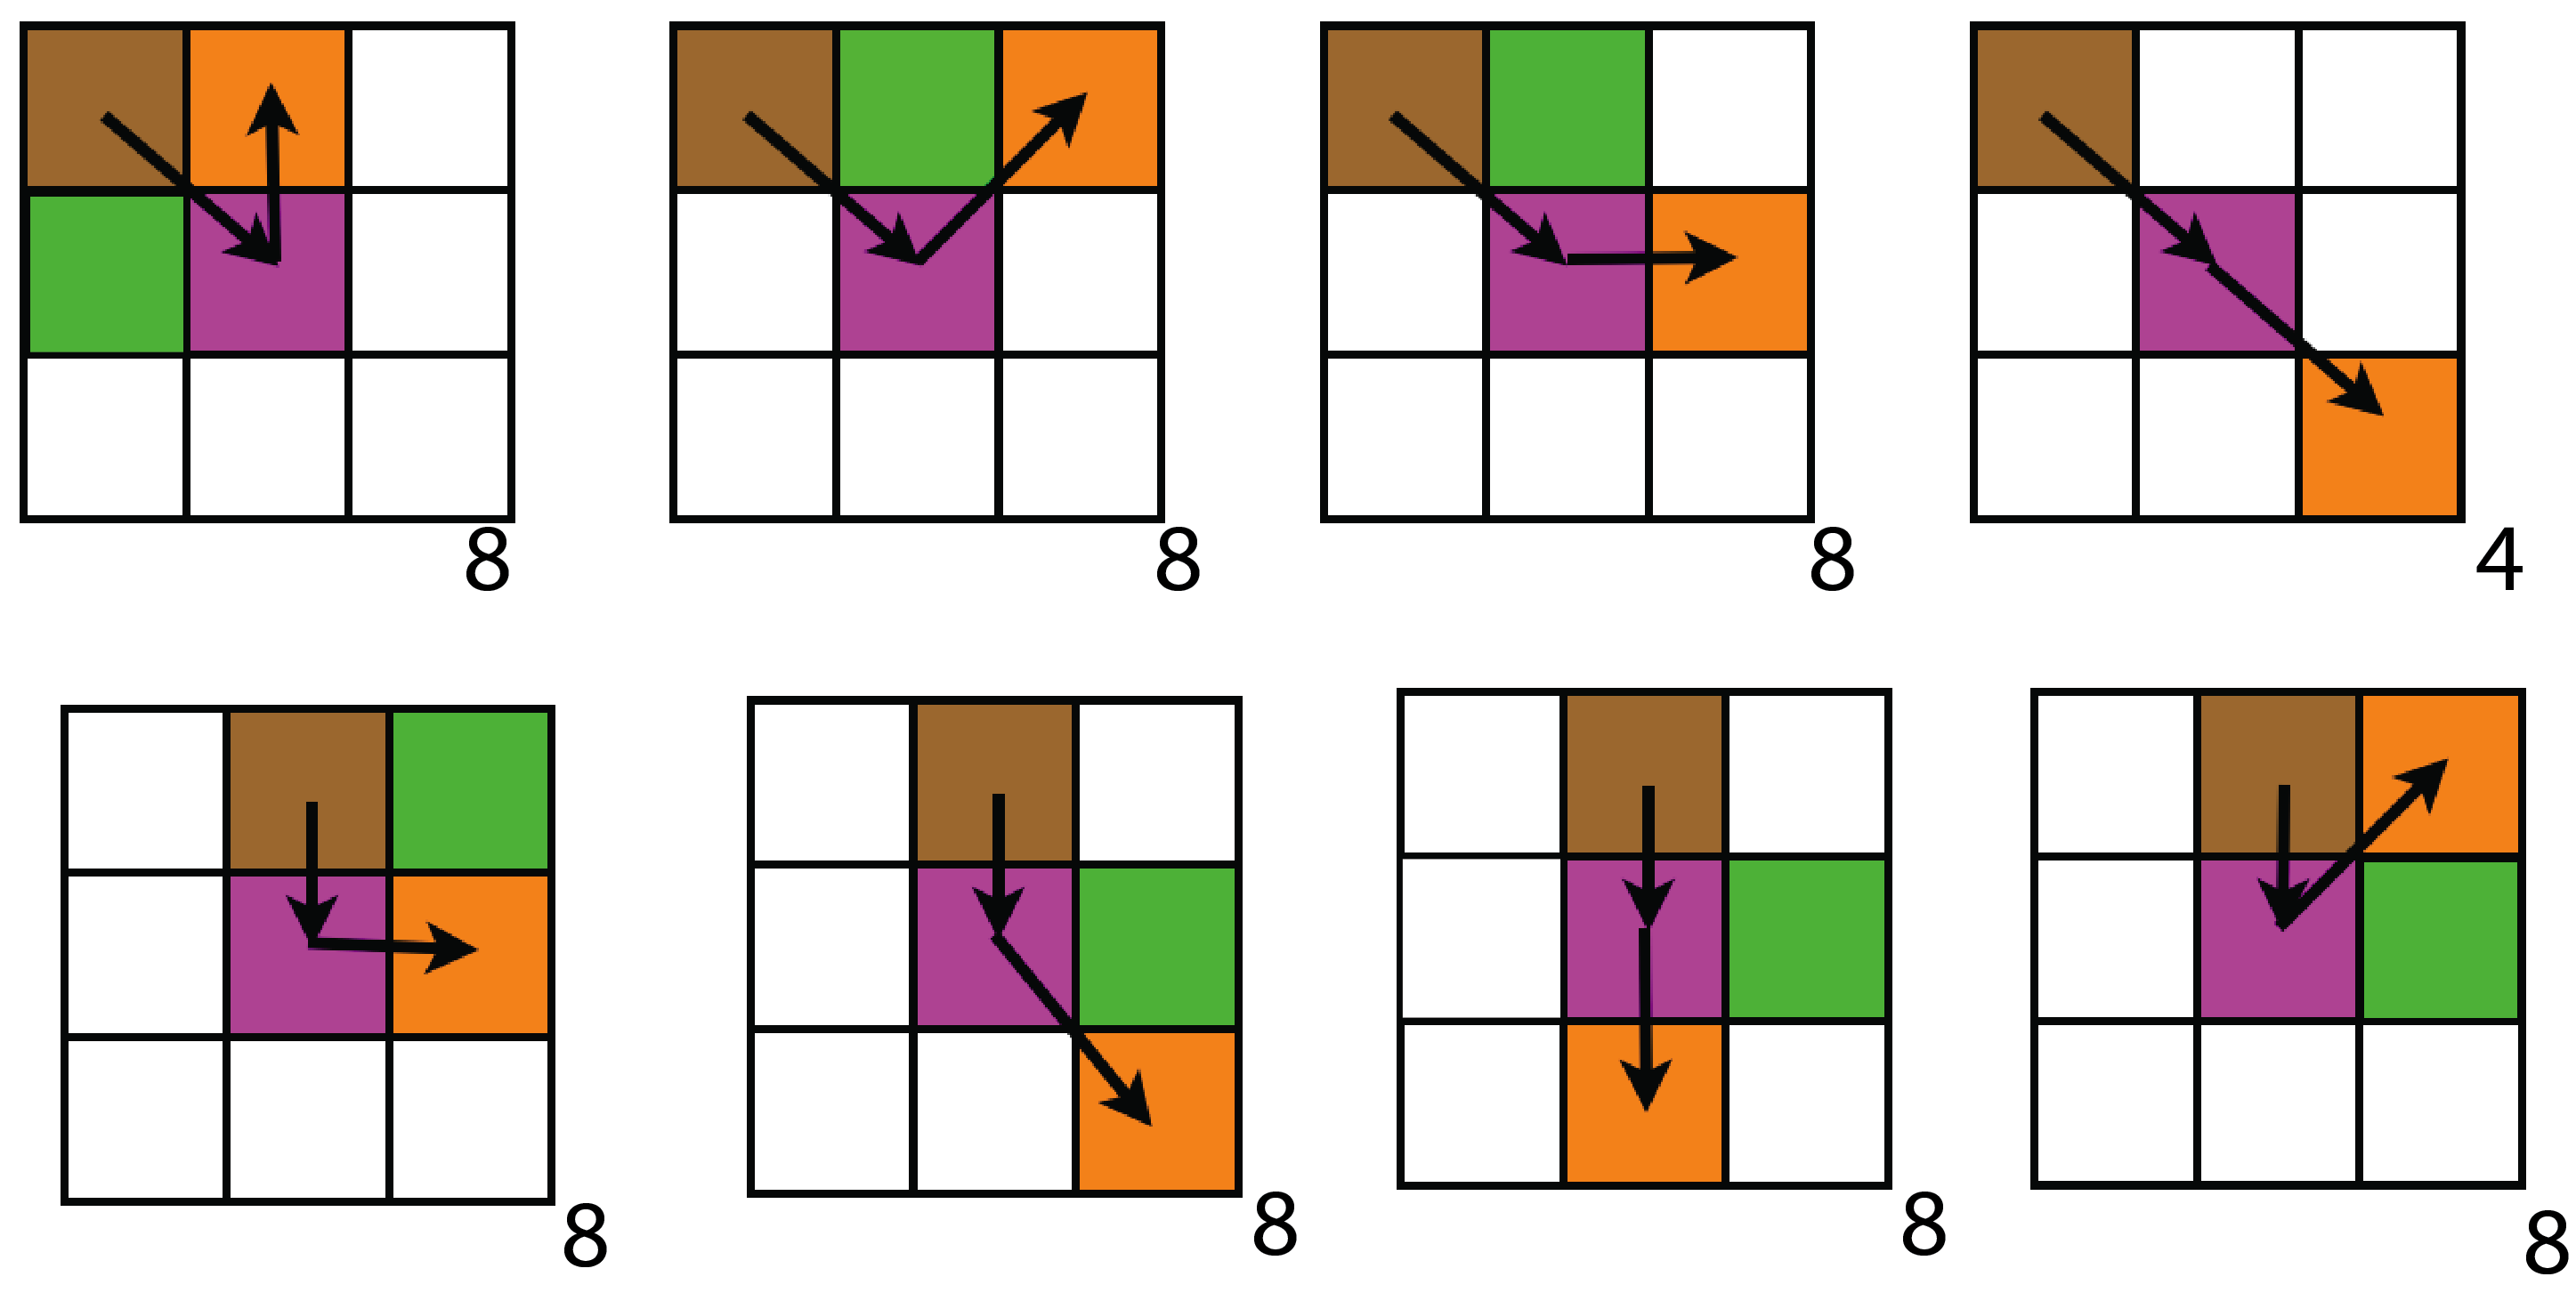
\includegraphics[width=\columnwidth]{Polymer.png}}
\caption{
\label{fig:polymer}
Configurations of upstream (brown) and downstream (orange) neighbors adjacent to a central cell (purple) and a mutually-adjacent neighbor (green) on a 2D lattice.
Numbers indicate the degeneracy of each configuration (via rotation and reflection).
There are 60 configurations in total.
}
\end{figure}

The implementation of each case requires several steps (including verifying the bidirectional bond integrities,
and checking the target cell is empty).
To illustrate the need for some of the ``frills'' in the core CA
(specifically indirect addressing and a Scheme-based assembler),
we observe that when using {\tt Load-Switch} and {\tt Load-Add-Store}
with no indirect addressing (the closest thing to lookup tables), the polymer program XML was 2.3Mb (52k gzipped).
With indirect addressing, this reduces to 127k (gzipped: 3k);
using the Scheme assembler, it is just 5k (gzipped: 1k).
Thus the Scheme assembler is, first and foremost, a compression strategy.

\subsection{RNA State Machines}

We model RNA as a two-tolerant random walk on the lattice\cite{LeoniVanderzande2003};
that is, up to two nucleotides can occupy a single cell, as long as they are base-paired
(Figure~\ref{fig:rna}).
In biochemistry, base-pairing is the mechanism whereby a nucleotide polymer pairs up to
a complementary version of itself, which e.g. leads to the double-stranded DNA molecule.
It is fundamental to the self-replicating ability of nucleotide sequences.

\begin{figure}
\fbox{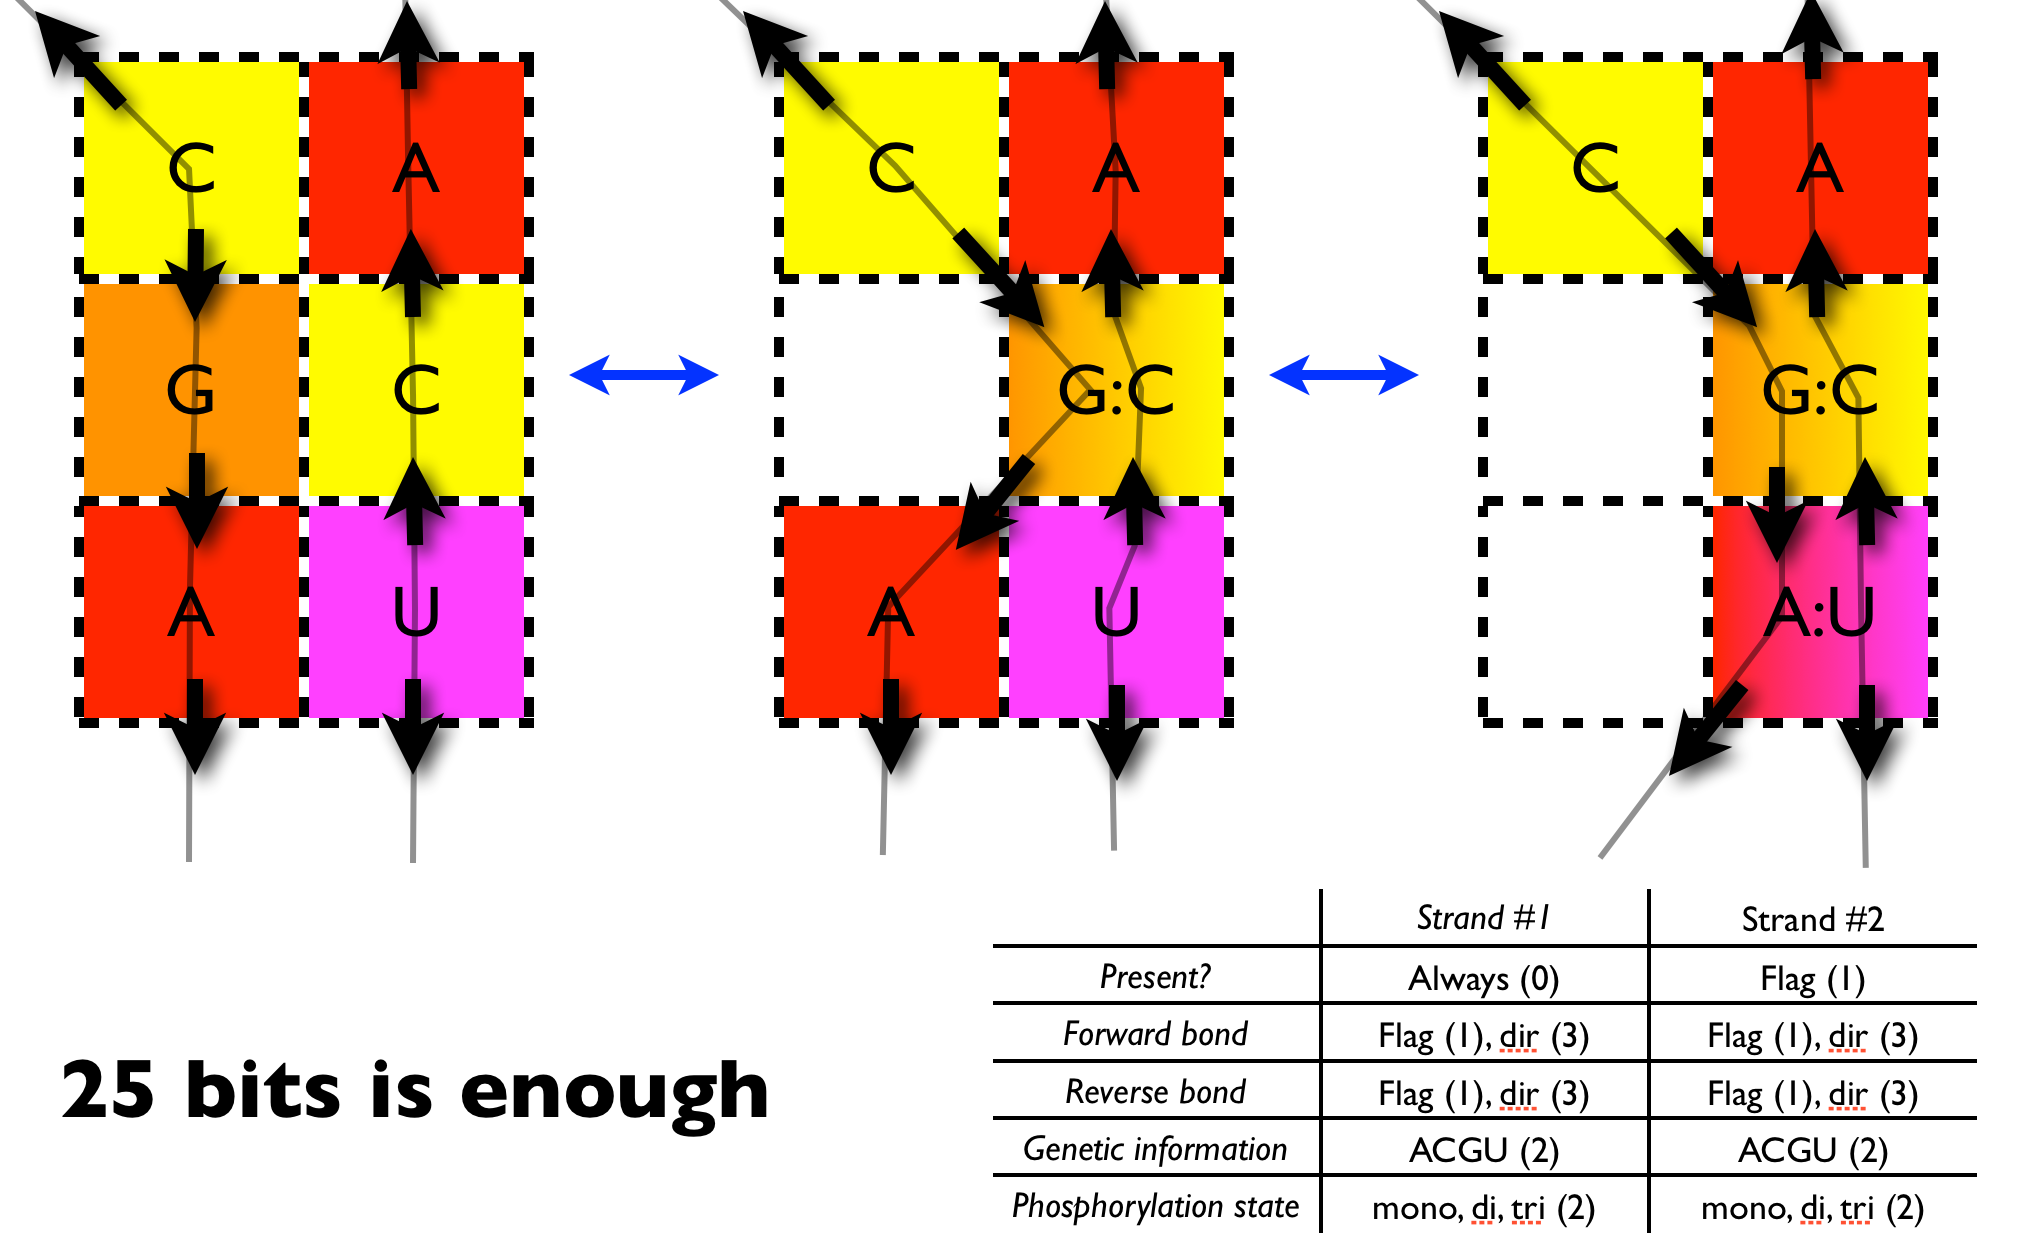
\includegraphics[width=\columnwidth]{RNA.png}}
\caption{
\label{fig:rna}
Base-pairing in the RNA model involves two nucleotides occupying the same cell, which then has up to four neighbor bonds.
}
\end{figure}

RNA basepair models require up to 4 bond directions and two base values to be stored in each cell.
The full range of bond configurations can be encoded in 16 bits/cell on the 2D lattice (23 bits/cell on the 3D lattice).
In practice it is convenient, albeit slightly more wasteful of bits,
to use distinct bitfields to encode the bond directions, presence/absence flags, and bases.
This requires 21 bits/cell on the 2D lattice, and 25 bits/cell on the 3D lattice.
% Activated phosphorylation states for each base can be recorded with another 2-4 bits.


\subsection{Agent State Machines}
\label{sec:AgentStateMachines}

PixelZoo also implements various agent models inspired by natural systems at longer-than-molecular length scales.
These include the bacterial tumble-run model of directed motion alternating with random walks\cite{RosserEtAl2013},
various forms of reaction-diffusion, directed diffusion, and diffusion-limited aggregation \cite{DLA},
the two-dimensional Ising model of magnetic spins \cite{Onsager1944},
the Lotka-Volterra predator-prey systems \cite{Lotka1910,Hirota199739},
ecological rock-paper-scissors games \cite{Tainaka2000},
forest fires \cite{Karafyllidis1997},
and lattice versions of the Wright-Fisher model of genetic drift \cite{MathiesonMcVean2013}.

% Ecosystem balancing and stability of food webs \cite{quince2005topological}.


\section{Game Design}

Rendering of the board uses an isometric view switching from monochromatic tiles (at distant zooms)
to sprites (at close zooms).

\subsection{Basic Play}

The background story involves terraforming planets from an orbital craft.
The game plays like an isometric painting program, but with live pixels.

The primary game goal is to maintain dynamic equilibrium inside a micelle
among a population of three chemical species in a rock-paper-scissors ecology.

\subsection{Network Play}

The multiplayer game is implemented using a RESTful server \cite{rest}.
The client posts a temporary lock on a board at the start of the player's turn,
and can then ``check out'' the board, saving it periodically during the turn.
Locks (and hence turns) are time-limited, and there is a minimum time between turns by the same player.
There are also daily limits on the particles that players can place on a board.

The competitive multiplayer goal is to keep your population alive under attack.
Keeping the population alive earns in-game money which can be spent designing new particles.

The mobile game client presents an interface for the player to
log in and out, browse worlds, pick a world, select terraforming tools, and play.

\subsection{Creating New Tools}

A player can post XML to server describing new particles and tools
(with restrictions; e.g. no Scheme code is allowed at present,
due partly to App Store prohibitions on downloaded code).

Creating and using new reaction-diffusion particles and spray-tools costs in-game money,
which can be earned by playing, or when others buy a player's tools.

\subsection{Implementation}

PixelZoo is implemented in Gnu C, libXML, GDataXML, ChibiScheme, XCode, and Perl Catalyst.
The prototype RNA CA was implemented in Java.

\section{Discussion}

PixelZoo implements polymers and RNA molecules,
and several other biologically-inspired agents, along with a mobile client prototype and multiplayer server infrastructure.
Planned work mostly involves creating new particle behaviors,
and adding game polish.

\subsection{Acknowledgements}

Many thanks are due Alex Shinn, Richard Evans, Michael Mateas, Sean Eddy, Gerald Joyce, Chris Quince,
and Rudy Rucker for help and inspiration.


\bibliography{pzpaper}

\balancecolumns
% That's all folks!
\end{document}
